%%%%%%%%%%%%%%%%%%%%%%%%%%%%%%%%%%%%%%%%%%%%%%%%%%%%%%%%%%%%%%%%
\documentclass[a4j,10pt,twocolumn]{jarticle}
\usepackage{ipsjz}           % 全国大会用パッケージ
\usepackage[dvips]{graphicx} % 図の取り込み用
\usepackage{siunitx}		 % SI単位
\usepackage{hyperref}
%%%%%%%%%%%%%%%%%%%%%%%%%%%%%%%%%%%%%%%%%%%%%%%%%%%%%%%%%%%%%%%%
%% タイトル
\title{3次元環境認識に基づく死角領域内のAR可視化による\par
ドローン操縦性向上} 
\etitle{Improving Drone Maneuverability by AR Visualization in Blind Spot Areas Based on 3D Environmental Awareness}   

%% 著者名
\author{竹内一真\DAG \quad 林聡一郎\DDAG \quad 上原夏紀\DDAG \quad 佐藤健哉\DDAG}
\eauthor{Kazuma Takeuchi\DAG, Soichiro Hayashi\DAG , Natsuki Uehara\DAG and Kenya Sato\DAG} 

%% 所属
\affiliation{\DAG 同志社大学理工学部情報システムデザイン学科\\ \DDAG 同志社大学大学院理工学研究科情報工学専攻}
\eaffiliation{\DAG Doshisha University}

%% メールアドレス
%\email{\{address1, address2, address3\}@cs.inf.shizuoka.ac.jp}

%%%%%%%%%%%%%%%%%%%%%%%%%%%%%%%%%%%%%%%%%%%%%%%%%%%%%%%%%%%%%%%%
\begin{document}
\maketitle              % 日本語タイトル作成
\makeetitle             % 英語タイトル作成
\baselineskip=1.55zh   %必要に応じて行間を調整

%---------------------------------------------------------------------
%---------------------------------------------------------------------
\section{はじめに}
近年,多方面でのドローンを活用した事業が進出しており,小型ドローンの特徴である小さな機体を活かして,人が入れない狭い空間での活躍の場も増えることが考えられる.しかし,狭小空間でのドローンの飛行は,遮蔽物が多く,遮られた視点からの操縦を必要とし,操縦は困難な場合がある.
\par
カメラ搭載のドローンを使用する場合では,操縦者はドローンから送られてくる映像を元に操縦が可能となる.そのような操縦方法によって,安全な距離から狭小空間を探索することができるが,カメラが前方しか写さないという点から一人称視点(FPV:First Person View)の操縦では前方以外の死角が多くなり,状況認識が不十分であり\cite{FPV},また,機体の大きさを掴めないという欠点がある.
\par
そこで,拡張現実を用いることで,操縦者の死角領域内を可視化し,狭小空間での操縦性の向上を検討する.

\section{ARを利用した障害物の知覚}
拡張現実を用いて,死角領域を飛行するドローンを操縦者視点で操縦することが可能となる.しかし,操縦者視点での操縦を実現する上で,障害物までの距離感が掴めない懸念がある.
% 自律飛行のドローンでの障害物回避に関する研究は数多くされているが,手動飛行の際,操縦者にどのように障害物を知覚させることが障害物への衝突を緩和できるかの研究はされていない.
また,自律飛行のドローンでの障害物回避は実現されているが,センサ搭載制限のある小型ドローンでは,障害物回避の支援がないため,衝突の危険性がある.
そこで本研究では,ARを用いることでドローンの操縦性を向上させるための直感的で視覚的な合図を提供することが可能である\cite{ARinterface}ことから,ドローン近傍の障害物を検知するAR方式を提案することで,操縦者にとってどのような情報が障害物までの距離感を把握し,安全にドローンを操縦できるかを検討した.
%---------------------------------------------------------------------
%---------------------------------------------------------------------
% \section{関連研究}
% \subsection{}
% Eratらの研究では\cite{drone},狭い場所でのドローン操縦が困難ということで,三人称視点のドローン操縦手法を提案している.ドローンがSLAM技術で空間マッピングをすることで,空間の仮想現実を構築し,閉鎖環境をみえるようにするというものである.しかし,走行の際に障害物にぶつからないように設定してあり,実際の狭小空間での危険性などが提示されていない問題があげられる.
% \subsection{概要}
% またMichaelらは\cite{interface},人間がドローンの動きの意図を視覚的に理解するため,ARを用いたユーザインタフェースデザインを作成し評価した.結果として,ドローンに対しARを用いた様々なデザインは,ARなしと比べ,課されたタスク効率を大幅に向上させ,ARを用いることでドローンの操縦性を向上させるための直感的で視覚的な合図を提供することが可能であることが示された.

%---------------------------------------------------------------------
\begin{figure}[t]
\begin{center}
  \scalebox{0.55}{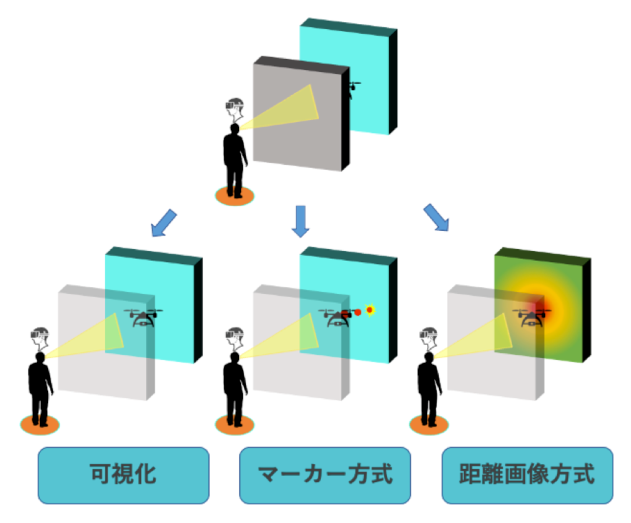
\includegraphics{img/overview.eps}}\vspace{-2mm}
  \caption{ARによるドローンの可視化}
  \label{fig:flow}
\end{center}
\end{figure}
%---------------------------------------------------------------------
\section{提案手法}
% 本章では,3次元環境認識に基づく死角領域内のAR可視化の概要について示す.
\subsection{概要}\label{}
本研究では,操縦者とドローンの間に遮蔽物があり,ドローンを視認できない環境を想定する.遮蔽物が存在すると判断した際,その遮蔽物を透過することで,操縦者への死角領域の空間認識を提供する.
また,死角領域内をドローンが飛行している際に,近傍の障害物までの距離が掴めない問題点を解決するために,2つのARインタフェース方式である距離画像方式,マーカー方式を開発する.
% \par
% 以降の節ではStereo,Markerの詳細について説明する.

\subsection{距離画像方式}
距離画像方式は,ステレオビジョンを参考にしており,ドローンから障害物までの距離に応じて,障害物の色を分けている.距離画像方式は,全体的な環境の理解を提供しており,ドローン周辺の障害物全ての衝突の危険性を示す.

\subsection{マーカー方式}
マーカー方式は,ドローンから見て最も近い障害物に対して,目印を付けている.距離画像方式では障害物全てが色分けされているため,操縦者を混乱させる可能性がある.マーカー方式では,最も危険な障害物だけを知覚させるため,距離画像方式に比べ簡易的なアプローチとなっている.

%---------------------------------------------------------------------
%---------------------------------------------------------------------

\section{評価}
\subsection{実装}
システム構成を図2に示す.
実際に使用したドローンはTello EDUであり,操作端末はMacBookProを用いる.ドローン未経験者と経験者による差を出さないために,ドローンの速度,一度に進む距離,旋回角度などは事前に設定している.
\par
ARHMDはMicrosoft HoloLens2を使用する.
事前にHoloLensのSpatial Mappingにより環境マッピングを行い,静的な3次元環境地図を作成する.
% ゲーム・アニメーションエンジンであるUnity内の3D仮想空間上で操縦者とUnity内の操縦者の位置合わせを行っている.

% この3次元環境地図とドローンを現実と同様の配置を行い,操縦者とUnity内の操縦者の位置合わせを行っている.
\par
サーバーではドローンの移動距離やピッチロールヨーをHoloLensに送信することで,3D仮想空間上に存在するドローンの位置合わせを行っている.
% \subsection{実装}
% Stereo,Markerでは共に障害物までの距離によって,危険度を色で示している.ドローンから障害物までの操縦者が危険な距離は を参考にしている.
% \par
% Stereoでは,障害物までの距離が0.5mまでを赤色で示し,0.5m~0.7mまでを黄色で示し,0.7m~1.0mまでを緑色で示している.
% \par
% Markerでは障害物までの距離が0.3m~0.5mの際に赤色のマーカーで示し,0.5m~0.7mの際に黄色のマーカーを示す.各デザインの色の使い分けにより,操縦者への視覚的支援を行う.

%---------------------------------------------------------------------
\begin{figure}[tb]
\begin{center}
  \scalebox{0.61}{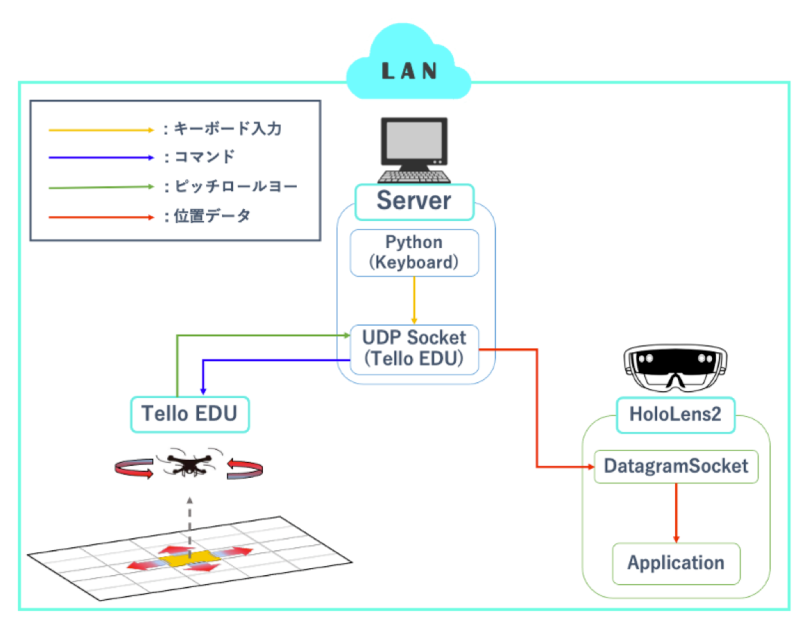
\includegraphics{img/flow.eps}}\vspace{-2mm}
  \caption{システム構成}
  \label{fig:principle}
\end{center}
\end{figure}
%---------------------------------------------------------------------

\subsection{実験}
% 実験環境を図4に示す.
% \begin{figure}[tb]
% \begin{center}
%   \scalebox{0.50}{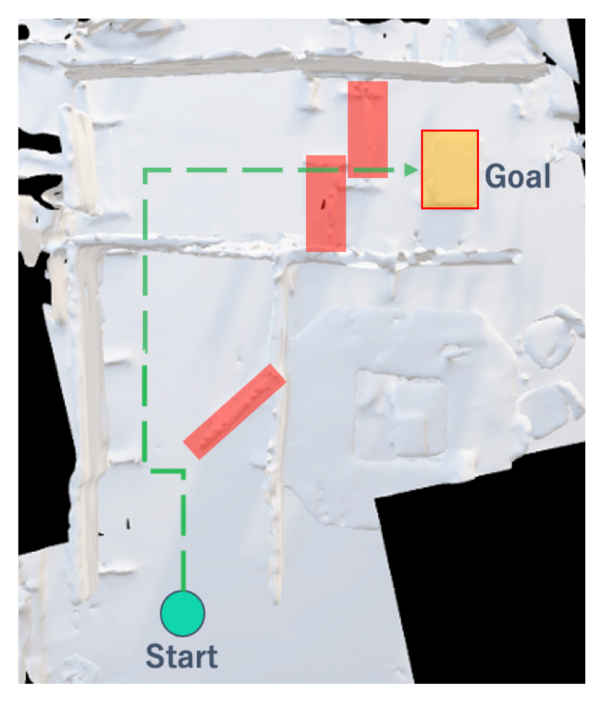
\includegraphics{img/exp.eps}}\vspace{-2mm}
%   \caption{実験環境}
%   \label{fig:principle}
% \end{center}
% \end{figure}
実験参加者はドローンをスタート地点から目的地まで操縦し,目的地点で着陸するタスクを行った.その間,衝突の恐れのある障害物を設置し,参加者にはぶつかることなく正確に通過することを要求した.実験では従来のドローン操縦,遮蔽物を可視化した手法,距離画像方式,マーカー方式の計4つの手法で実験を行った.また,操縦者がドローンを操縦する際の衝突する危険性がある距離が0.3mと示されている\cite{obstruct}ため,0.3mを操縦者への危険告知の閾値とした.
% \par
% また,予備実験で,慣れにより実験後半の操縦時間が速くなったり,ARの経験がないことから戸惑いが生じ,初めの操縦時間が長くなることがわかった.今回は,この効果を消すために,ドローン操縦を5〜10分ほど練習させた後に,各手法で実験環境を1度走行させることで,練習量を増やした.

%---------------------------------------------------------------------
\subsection{評価と考察}
各手法での,ドローンがスタート地点から目的地に着陸し停止するまでの操縦時間,障害物への衝突回数,参加者へのアンケートを記録した.その結果,ARを利用した手法ではARなしと比べ,平均の操縦時間が約1分減少し,衝突回数は約2回減少し,一貫して操縦時間と衝突回数共に低かったことがわかった.アンケートの結果では,操縦者にとってARを利用した死角領域内を可視化した方式は視認性を向上させ,ドローン操縦性を向上させたことが分かった.特に距離画像方式では操縦時間の短縮が見られた.これはドローン周辺の障害物全ての危険度が把握できることより,操縦者への安心感を向上させた.
%---------------------------------------------------------------------
\begin{figure}[tb]
\begin{center}
  \scalebox{0.45}{\includegraphics{img/marker.eps}}\vspace{-2mm}
  \caption{マーカー方式}
  \label{fig:principle}
\end{center}
\end{figure}
%---------------------------------------------------------------------

\section{まとめ}
小型ドローンでの遮られた視点からの狭小空間での操縦は死角の多さや,ドローンと障害物までの距離感が測れないことが懸念されている.本研究では操縦者の死角領域内に存在するドローンと周辺を可視化し,ドローン周辺の障害物を知覚するためのAR方式を提案し,実験を行うことで,遮られた視点からの狭小空間でのドローン操縦性を評価した.結果として,ARを利用した手法では実験環境での操縦時間が短く,衝突回数も少なかったことから操縦性の向上が確認された.
また,障害物を知覚するためのAR方式では,ドローン周辺の障害物に危険度を振り分けている手法が,操縦者への安心を与え,操縦性を向上させたことが確認できた.

\vspace{10pt}
本研究の一部はJSPS科研費20H00589の助成を受けたものである.
%---------------------------------------------------------------------
%---------------------------------------------------------------------
{\footnotesize 

% \bibliography{reference}
% \bibliographystyle{junsrt}

\begin{thebibliography}{99}
\bibitem{FPV}
Green, S. A., Chase, J. G., Chen, X. and Billinghurst, M.: Evaluating the Augmented Reality Human-Robot Collaboration System, 2008 15th International Conference on Mechatronics and Machine Vision in Practice, Auckland, pp. 521-526 (2008).
\bibitem{ARinterface}
Walker, M., Hedayati, H., Lee, J., and Szafir, D.: Communicating robot
motion intent with augmented reality, in HRI, pp. 316–324 (2018).

\bibitem{obstruct}
山田開斗,薄羽大樹,宮下芳明:ドローン操縦におけるクロッシング評価,研究報告ヒューマンコンピュータインタラクション(HCI),Issue.2,No.2,pp.1-6 (2019).

\end{thebibliography}
}
\end{document}
